\documentclass[fleqn]{article}
\usepackage[margin=1in]{geometry}
\usepackage[nodisplayskipstretch]{setspace}
\usepackage{amsmath, nccmath, bm}
\usepackage{amssymb}
\usepackage{enumitem}
\usepackage{graphicx}
\usepackage{float}
\usepackage{listings}
\usepackage{hyperref}
\usepackage[svgnames]{xcolor}
\graphicspath{
{./images}
{./images/nand}
{./images/nand/delay}
{./images/nand/design}
{./images/nand/noise_analysis}
{./images/nand/power}
{./images/nand/vtc}
{./images/nor}
{./images/nor/delay}
{./images/nor/design}
{./images/nor/noise_analysis}
{./images/nor/power}
{./images/nor/vtc}}

\hypersetup{
    colorlinks=true,
    linkcolor=black,
    filecolor=black,      
    urlcolor=blue
    }

\newcommand{\zerodisplayskip}{
	\setlength{\abovedisplayskip}{0pt}%
	\setlength{\belowdisplayskip}{0pt}%
	\setlength{\abovedisplayshortskip}{0pt}%
	\setlength{\belowdisplayshortskip}{0pt}%
	\setlength{\mathindent}{0pt}}
	
\definecolor{vgreen}{RGB}{104,180,104}
\definecolor{vblue}{RGB}{49,49,255}
\definecolor{vorange}{RGB}{255,143,102}

\lstdefinestyle{verilog-style}
{
    language=Verilog,
    basicstyle=\small\ttfamily,
    keywordstyle=\color{vblue},
    identifierstyle=\color{black},
    commentstyle=\color{vgreen},
    numbers=left,
    numberstyle=\tiny\color{black},
    numbersep=10pt,
    tabsize=8,
    moredelim=*[s][\colorIndex]{[}{]},
    literate=*{:}{:}1
}

\lstset{style={verilog-style},showstringspaces=false}

\makeatletter
\newcommand*\@lbracket{[}
\newcommand*\@rbracket{]}
\newcommand*\@colon{:}
\newcommand*\colorIndex{%
    \edef\@temp{\the\lst@token}%
    \ifx\@temp\@lbracket \color{black}%
    \else\ifx\@temp\@rbracket \color{black}%
    \else\ifx\@temp\@colon \color{black}%
    \else \color{vorange}%
    \fi\fi\fi
}
\makeatother

\newcommand{\code}[1]{%
	\colorbox{Gainsboro}{\texttt{#1}}%
}

\title{Lab 1}
\author{Owen Sowatzke}
\date{March 17, 2025}

\begin{document}

	% \offinterlineskip
	% \setlength{\lineskip}{12pt}
	% \zerodisplayskip
	\maketitle
	
	\section{Introduction}
	
	\section{Procedure}
	
	\section{Results}
	
	\subsection{First Order Transistor Model}
	
	\texttt{let ids=-vds\#branch}
	
	\texttt{let ids\_p=deriv(ids)}
	
	\texttt{plot ids\_p}
	
	\texttt{let ids\_pp=deriv(ids\_p)}
	
	\texttt{meas dc m max ids\_pp}
	
	\texttt{meas dc vgs\_i max\_at ids\_pp}
	
	\texttt{meas dc ids\_p\_i find ids\_p when vgs=vgs\_i}
	
	\texttt{let b = ids\_p\_i - m*vgs\_i}
	
	\texttt{let vt = -b/m}
	
	\texttt{print vt}
	
	\texttt{let ids\_p\_fit = m*vgs + b}
	
	\texttt{plot ids\_p ids\_p\_fit yrange}
	
	\begin{center}
	\label{table::nmos_params}
	\begin{tabular}{| c | c |}
		\hline
		Parameter & Value \\
		\hline	
		$V_{t0}$ & $0.6613 V$\\
		\hline	
		$V_{dsat}$ & $0.3948 V$\\
		\hline	
		$\lambda$ & $0.1289 V^{-1}$\\
		\hline			
		$k_n$ & $164.1 {\mu}A/V^2$ \\
		\hline
	\end{tabular}
	\end{center}
	
	\begin{center}
	\begin{tabular}{| c | c |}
		\hline
		Parameter & Value \\
		\hline	
		$V_{t0}$ & $-0.5765 V$\\
		\hline	
		$V_{dsat}$ & $-0.7988 V$\\
		\hline	
		$\lambda$ & $-0.3408 V^{-1}$\\
		\hline			
		$k_n$ & $28.48 {\mu}A/V^2$ \\
		\hline
	\end{tabular}
	\end{center}
	
	\subsection{NAND Gate}
	
	\subsubsection{Design}
	
	The pull-down circuit of the NAND gate is composed of two sequential NMOS gates. The pull-up circuit is the complement and is composed of two parallel PMOS gates. Note that we also increase the width of the PMOS transistor by a factor of 2 to account for the lower mobility of holes in the p-type material. The schematic for the resulting circuit is shown in Figure \ref{fig::nand_schematic}.
	
	\begin{figure}[H]
		\centerline{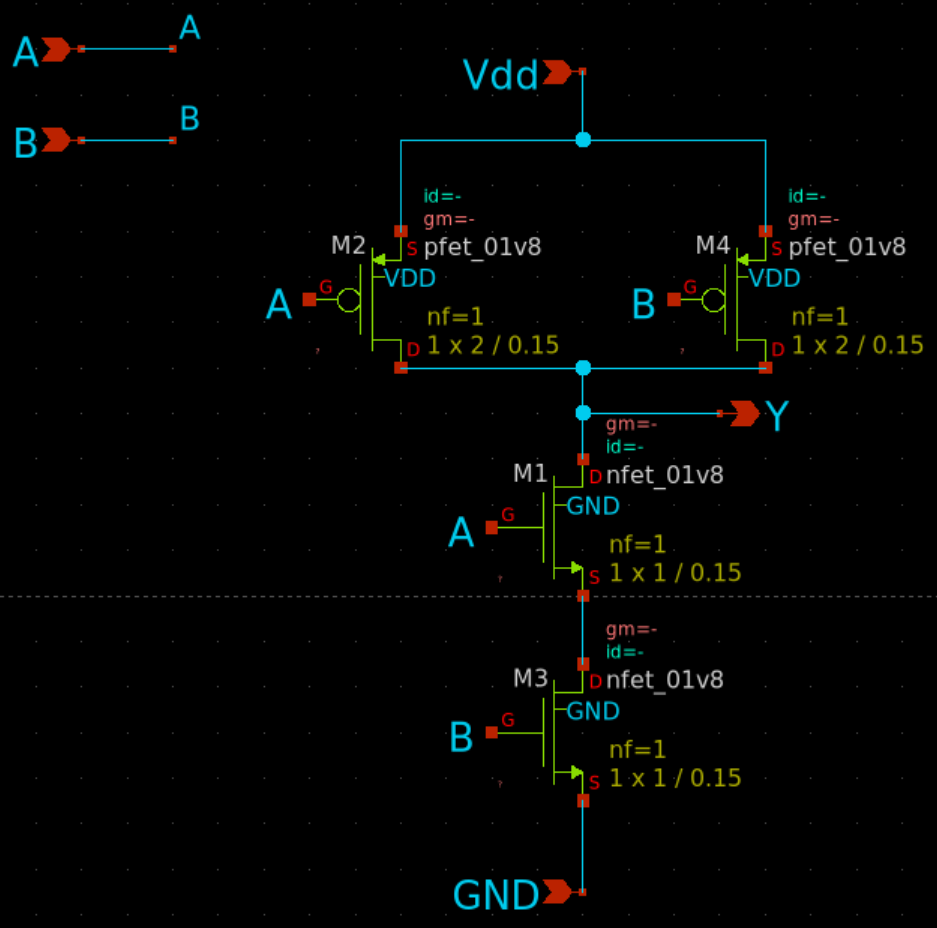
\includegraphics[width=0.4\textwidth]{nand_schematic.png}}
		\caption{NAND Circuit Schematic}
		\label{fig::nand_schematic}
	\end{figure}

	We also create a circuit symbol for the NAND gate, which is shown in Figure \ref{fig::nand_symbol}.
	
	\begin{figure}[H]
		\centerline{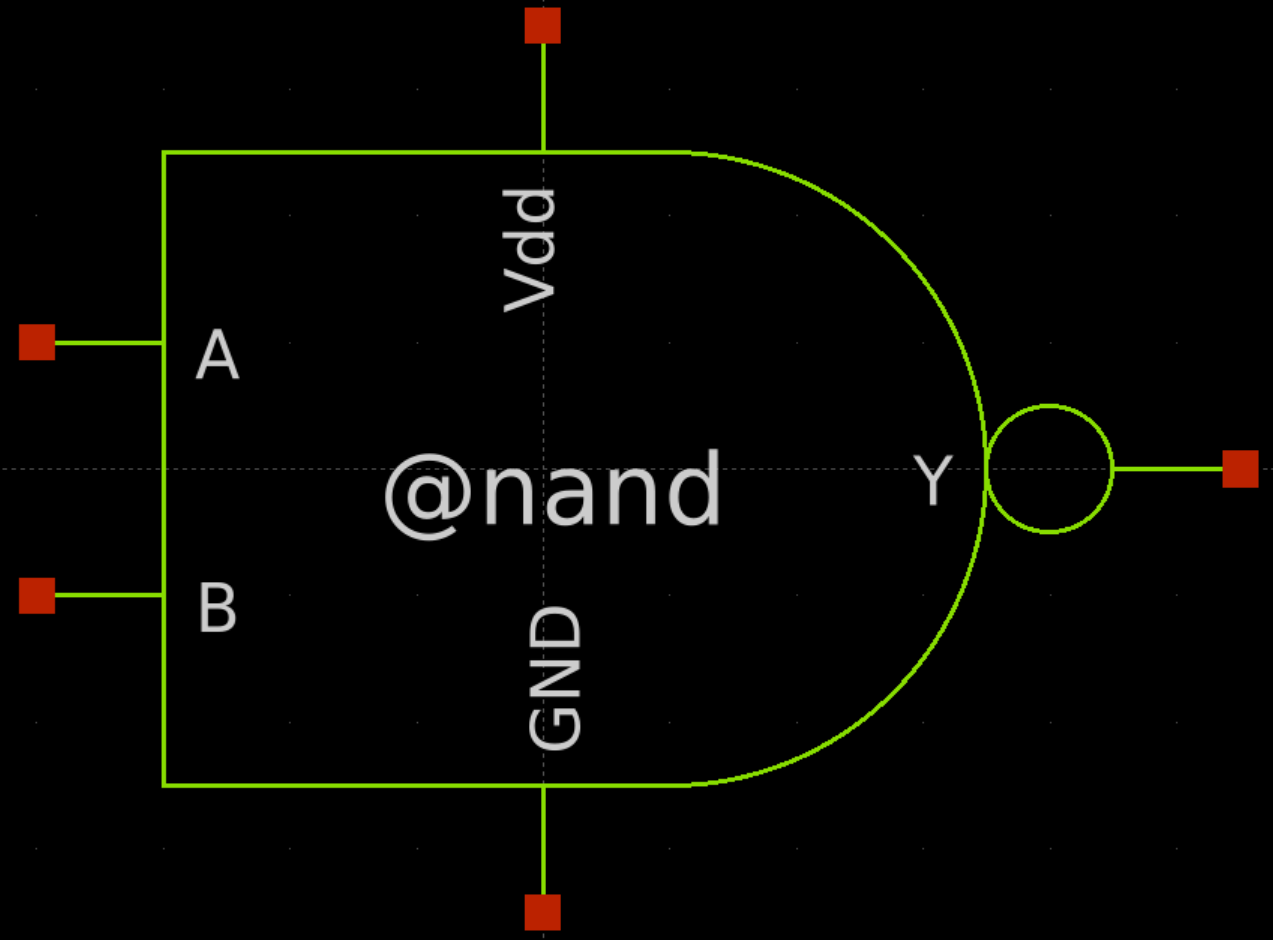
\includegraphics[width=0.4\textwidth]{nand_symbol.png}}
		\caption{NAND Circuit Symbol}
		\label{fig::nand_symbol}
	\end{figure}
	
	\subsubsection{Voltage Transfer Characteristics}
	
	In this section, we analyze the voltage transfer characteristics (VTC) of our NAND gate. For this analysis, we analyze the VTC when varying \texttt{a} and \texttt{b} independently and when varying \texttt{a} and \texttt{b} together. The test circuit we use when just varying the input \texttt{a} is included in Figure \ref{fig::nand_vtc_test_sweep_va}.
	
	\begin{figure}[H]
		\centerline{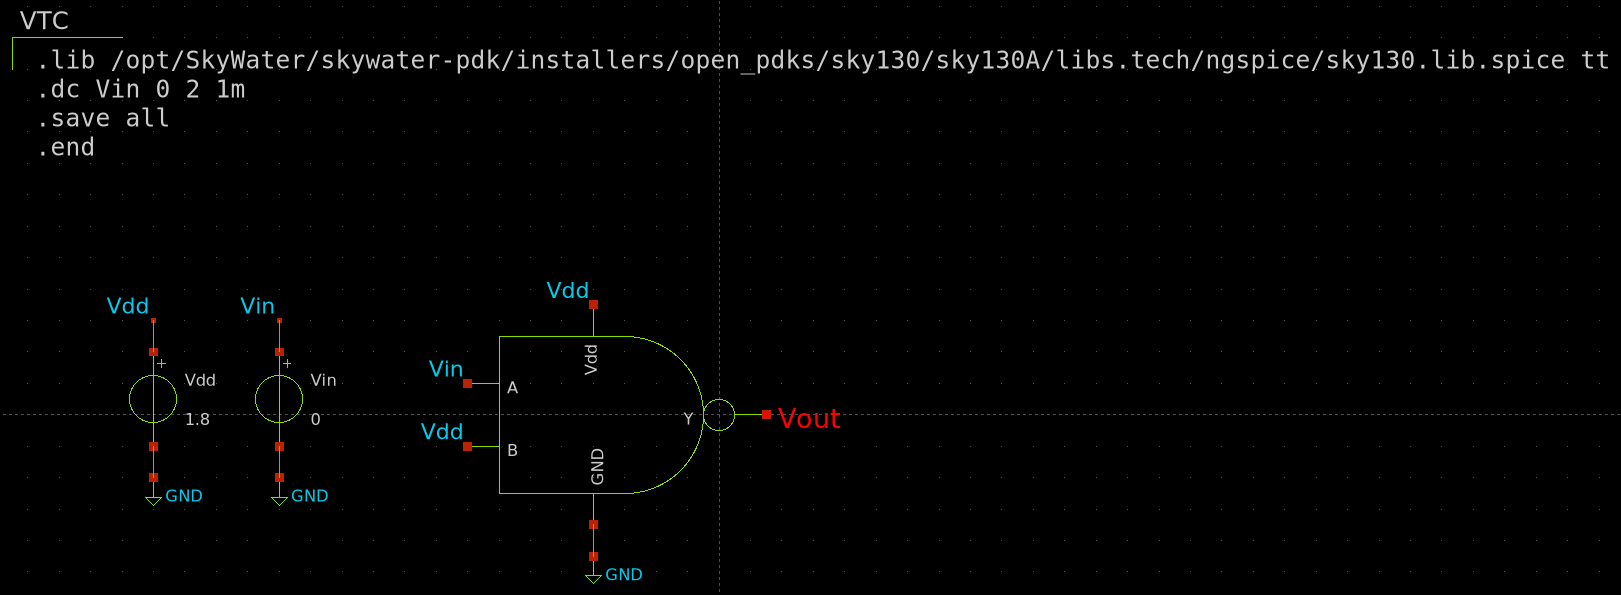
\includegraphics[width=0.8\textwidth]{nand_vtc_test_sweep_va.png}}
		\caption{NAND VTC Test Circuit for Independent Variations of Input \texttt{a}}
		\label{fig::nand_vtc_test_sweep_va}
	\end{figure}
	
	Using this test circuit, we perform DC analysis to determine the VTC and find \texttt{Va}, which is the voltage at which \texttt{Vin = Vout}. The results of this analysis are shown in Figure \ref{fig::nand_vtc_sweep_va}.
	
	\begin{figure}[H]
		\centerline{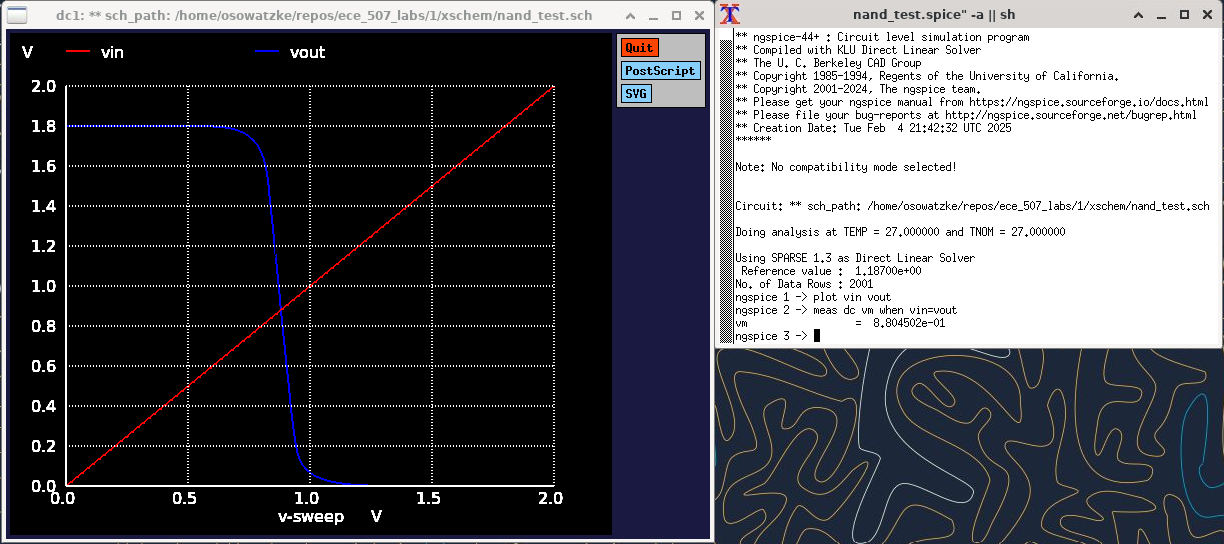
\includegraphics[width=0.8\textwidth]{nand_vtc_sweep_va.png}}
		\caption{NAND VTC Results for Independent Variations of Input \texttt{a}}
		\label{fig::nand_vtc_sweep_va}
	\end{figure}
	
	Examining the results, we find that \texttt{Vm = 0.8805V}. We perform similar analysis for independent variations of the input \texttt{b}. The test circuit and results are attached in figures \ref{fig::nand_vtc_test_sweep_vb} and \ref{fig::nand_vtc_sweep_vb} independently.
	
	\begin{figure}[H]
		\centerline{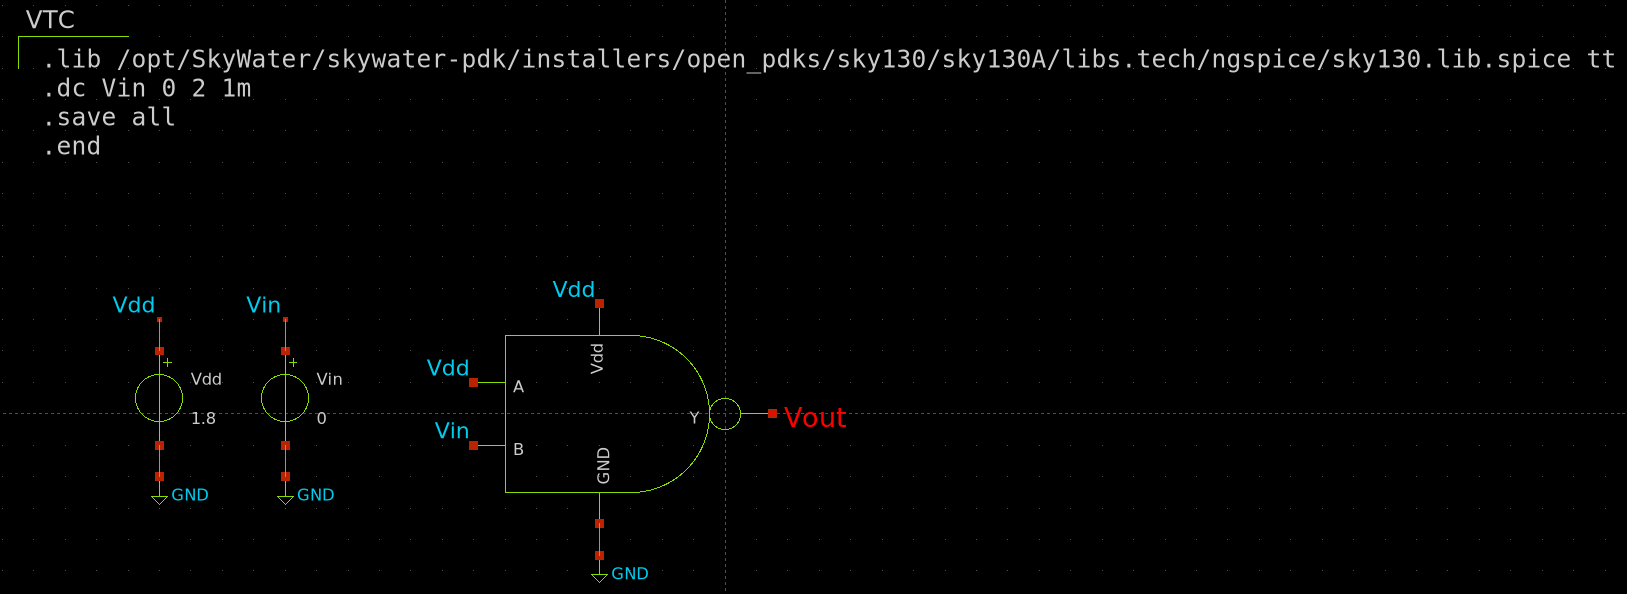
\includegraphics[width=0.8\textwidth]{nand_vtc_test_sweep_vb.png}}
		\caption{NAND VTC Test Circuit for Independent Variations of Input \texttt{b}}
		\label{fig::nand_vtc_test_sweep_vb}
	\end{figure}
	
	\begin{figure}[H]
		\centerline{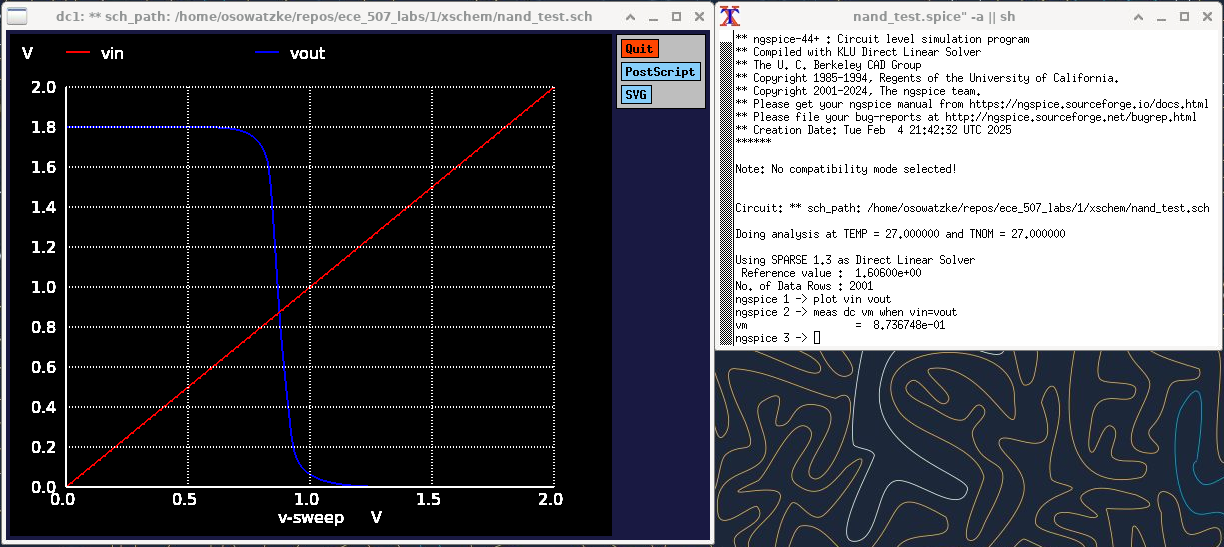
\includegraphics[width=0.8\textwidth]{nand_vtc_sweep_vb.png}}
		\caption{NAND VTC Results for Independent Variations of Input \texttt{b}}
		\label{fig::nand_vtc_sweep_vb}
	\end{figure}
	
	Examining the results, we find that \texttt{Vm = 0.8737V}. Finally, we sweep both inputs \texttt{a} and \texttt{b} together. The test circuit and results for this analysis are included in Figures \ref{fig::nand_vtc_test_sweep_va_vb} and \ref{fig::nand_vtc_sweep_va_vb} respectively.
	
	\begin{figure}[H]
		\centerline{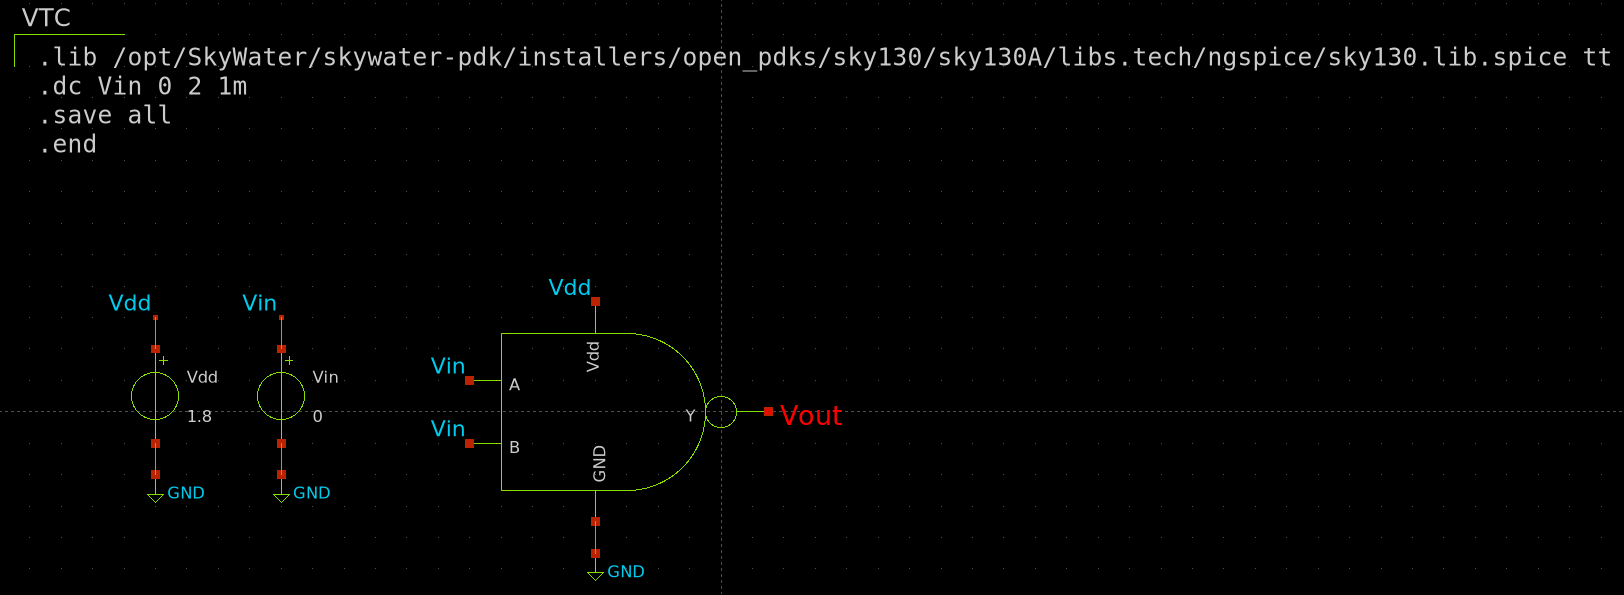
\includegraphics[width=0.8\textwidth]{nand_vtc_test_sweep_va_vb.png}}
		\caption{NAND VTC Test Circuit for Joint Variations of Inputs \texttt{a} and \texttt{b}}
		\label{fig::nand_vtc_test_sweep_va_vb}
	\end{figure}
	
	\begin{figure}[H]
		\centerline{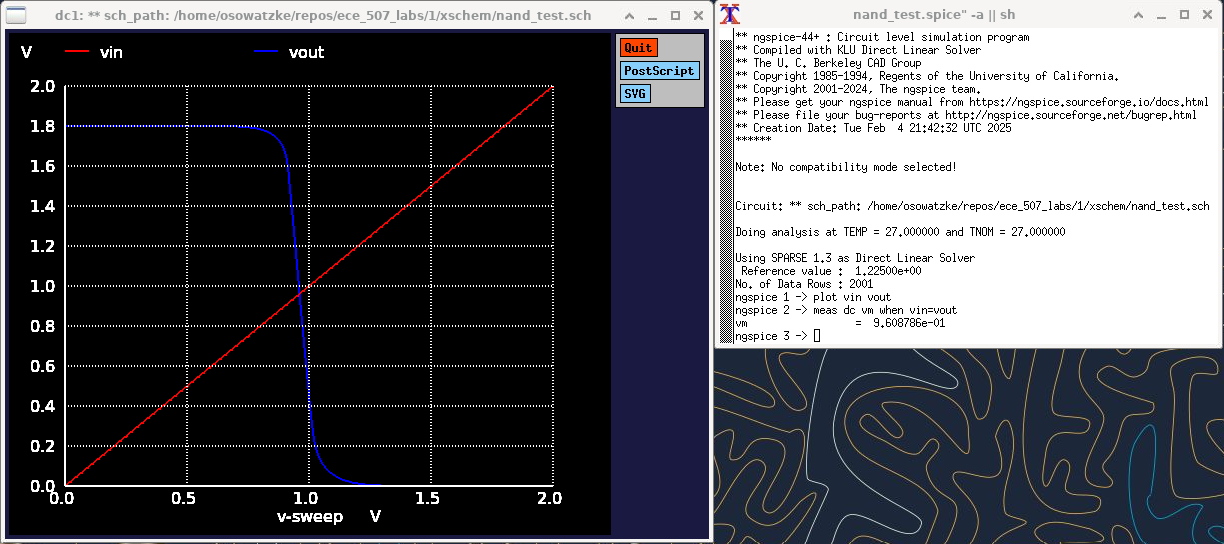
\includegraphics[width=0.8\textwidth]{nand_vtc_sweep_va_vb.png}}
		\caption{NAND VTC Results for Joint Variations of Inputs \texttt{a} and \texttt{b}}
		\label{fig::nand_vtc_sweep_va_vb}
	\end{figure}
	
	Examining the results, we find that \texttt{Vm = 0.9609V}.
	
	\subsubsection{Noise Analysis}
	
	Using the test circuits shown in Figures \ref{fig::nand_vtc_test_sweep_va}, \ref{fig::nand_vtc_test_sweep_vb}, and \ref{fig::nand_vtc_test_sweep_va_vb}, we perform noise analysis. We specifically use the test circuits to measure the noise margins, which are defined follows:
	
	\begin{equation}
		NM_H = V_{DD} - V_{IH}
	\end{equation}
	
	\begin{equation}
		NM_L = V_{IL} - GND
	\end{equation}
	
	In the above formulas, $V_{IH}$ and $V_{IL}$ are defined as the unity points of the gain function, where the gain is defined as the derivative of the VTC. For the case in which we only vary the input \texttt{a}, we can identify the unity gain points and the corresponding noise margins as follows:
	
	\begin{figure}[H]
		\centerline{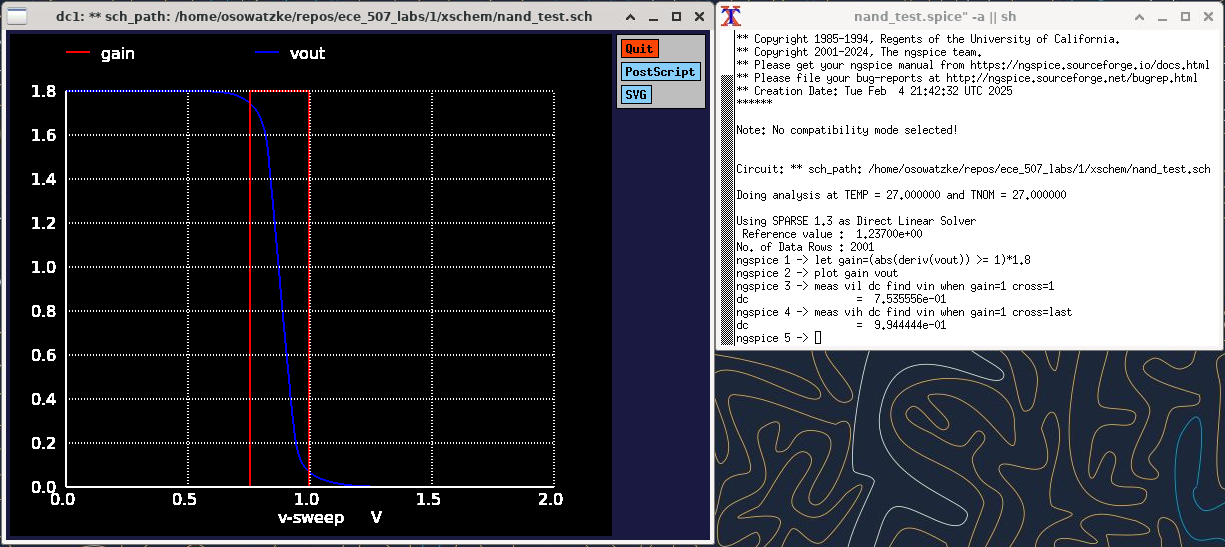
\includegraphics[width=0.8\textwidth]{nand_noise_analysis_sweep_va.png}}
		\caption{Measuring \texttt{Vil} for the NAND Gate when Input Variations are Limited to Input \texttt{a}}
		\label{fig::nand_noise_analysis_sweep_va}
	\end{figure}
	
	Examining the ngspice outputs, we find that \texttt{Vil = 0.7536 V} and \texttt{Vih = 0.9944 V}. This implies that \texttt{Nmh = 1.8 V - 0.9944 V = 0.8056 V} and \texttt{Nml = 0.7536 V}. We can repeat this analysis for independent variations of input \texttt{a} and for joint variations of inputs \texttt{a} and \texttt{b}. The ngspice outputs for this analysis are included in Figure \ref{fig::nand_noise_analysis_sweep_vb} and \ref{fig::nand_noise_analysis_sweep_va_vb}.
	
	\begin{figure}[H]
		\centerline{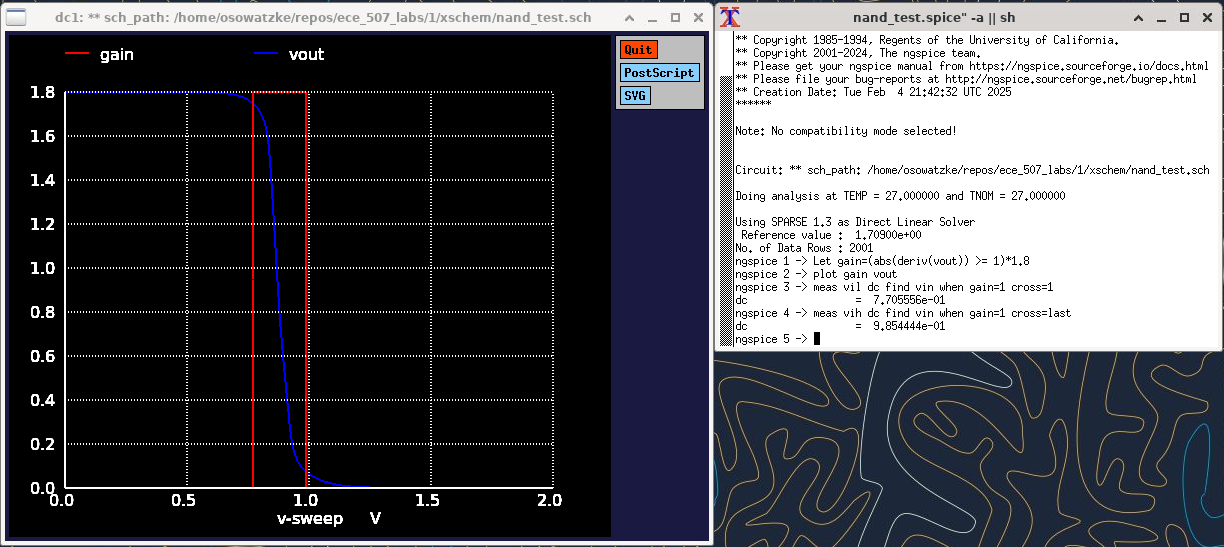
\includegraphics[width=0.8\textwidth]{nand_noise_analysis_sweep_vb.png}}
		\caption{Measuring \texttt{Vil} for the NAND Gate when Input Variations are Limited to Input \texttt{b}}
		\label{fig::nand_noise_analysis_sweep_vb}
	\end{figure}
	
	\begin{figure}[H]
		\centerline{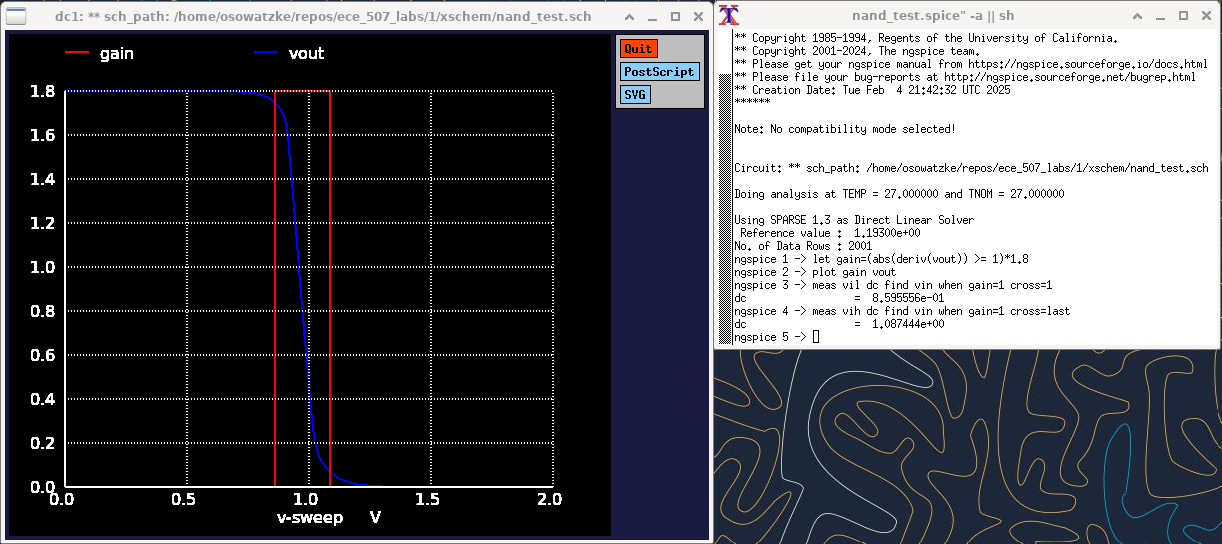
\includegraphics[width=0.8\textwidth]{nand_noise_analysis_sweep_va_vb.png}}
		\caption{Measuring \texttt{Vil} for the NAND Gate when Inputs \texttt{a} and \texttt{b} are Varied Together}
		\label{fig::nand_noise_analysis_sweep_va_vb}
	\end{figure}
	
	Examining the outputs, we find that the noise margins are defined as \texttt{Nmh = 0.8146 V} and \texttt{Nml = 0.7706 V} when input variations are limited to input \texttt{b}. When we vary the inputs \texttt{a} and \texttt{b} in unison, we find that the noise margins are \texttt{Nmh = 0.7126 V} and \texttt{Nml = 0.8596 V}.
	
	\subsubsection{Delay Analysis}
	
	In this section, we analyze the delay of the NAND gate and specifically measure the high to low propagation delay (\texttt{tphl}). To perform this analysis for independent variations of the input \texttt{a}, we use the following test circuit:
	
	\begin{figure}[H]
		\centerline{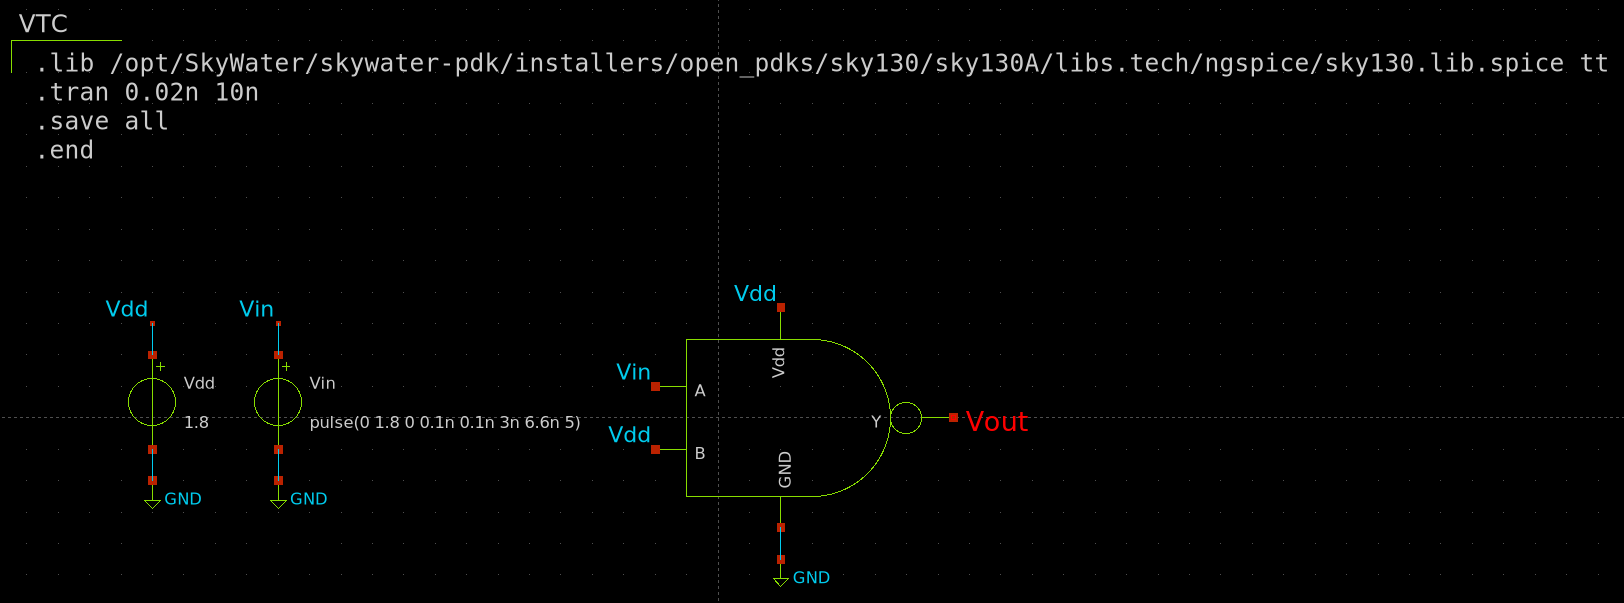
\includegraphics[width=0.8\textwidth]{nand_delay_test_sweep_va.png}}
		\caption{Test Circuit to Measure the Delay of the NAND Gate when Only Input \texttt{a} is Varied}
		\label{fig::nand_delay_test_sweep_va}
	\end{figure}
	
	Using the test circuit, we measure can measure the high-to-low propagation delay as follows:
	
	\begin{figure}[H]
		\centerline{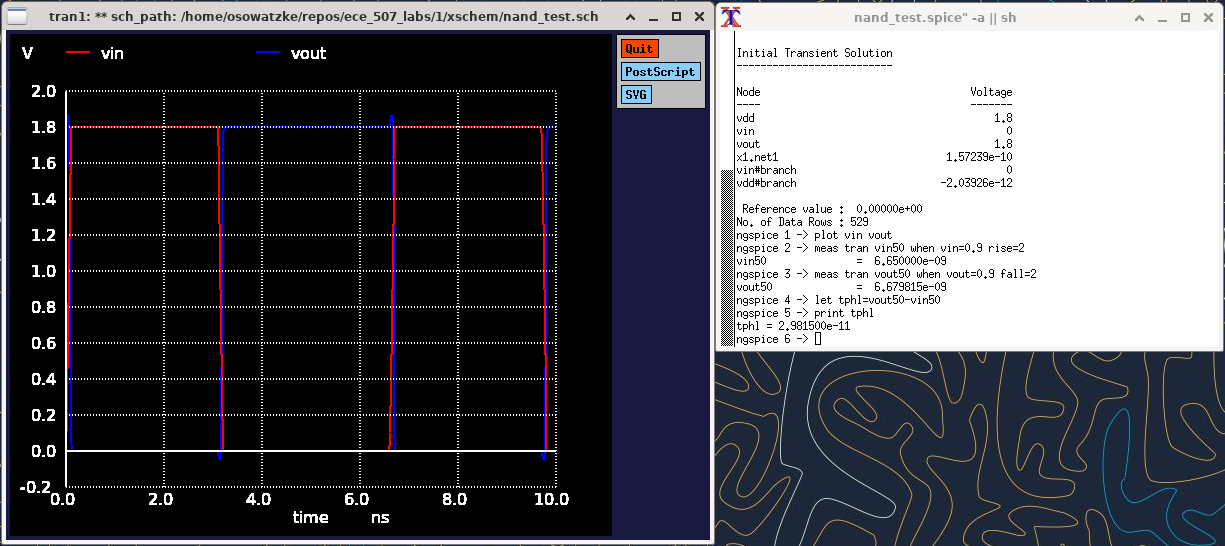
\includegraphics[width=0.8\textwidth]{nand_delay_sweep_va.png}}
		\caption{\texttt{tphl} Measurement for the NAND Gate when Input Variations are Limited to Input \texttt{a}}
		\label{fig::nand_delay_sweep_va}
	\end{figure}
	
	Examining the output results, we find that \texttt{tphl = 29.815 ps}. We can perform similar analysis to examine the impact of varying just the input \texttt{b}. The test circuits for this analysis is shown in Figures \ref{fig::nand_delay_test_sweep_vb} and the results are shown in Figure \ref{fig::nand_delay_sweep_vb}.
	
	\begin{figure}[H]
		\centerline{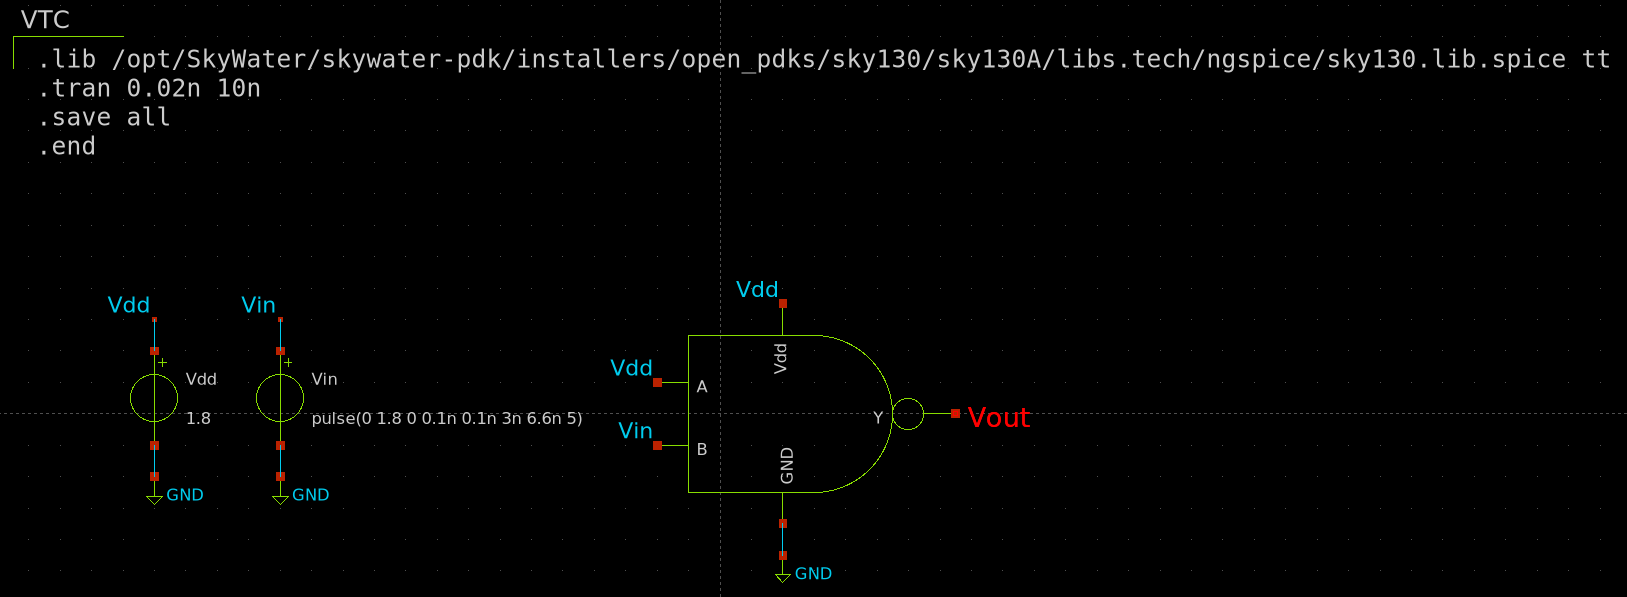
\includegraphics[width=0.8\textwidth]{nand_delay_test_sweep_vb.png}}
		\caption{Test Circuit to Measure the Delay of the NAND Gate when Only Input \texttt{b} is Varied}
		\label{fig::nand_delay_test_sweep_vb}
	\end{figure}
	
	\begin{figure}[H]
		\centerline{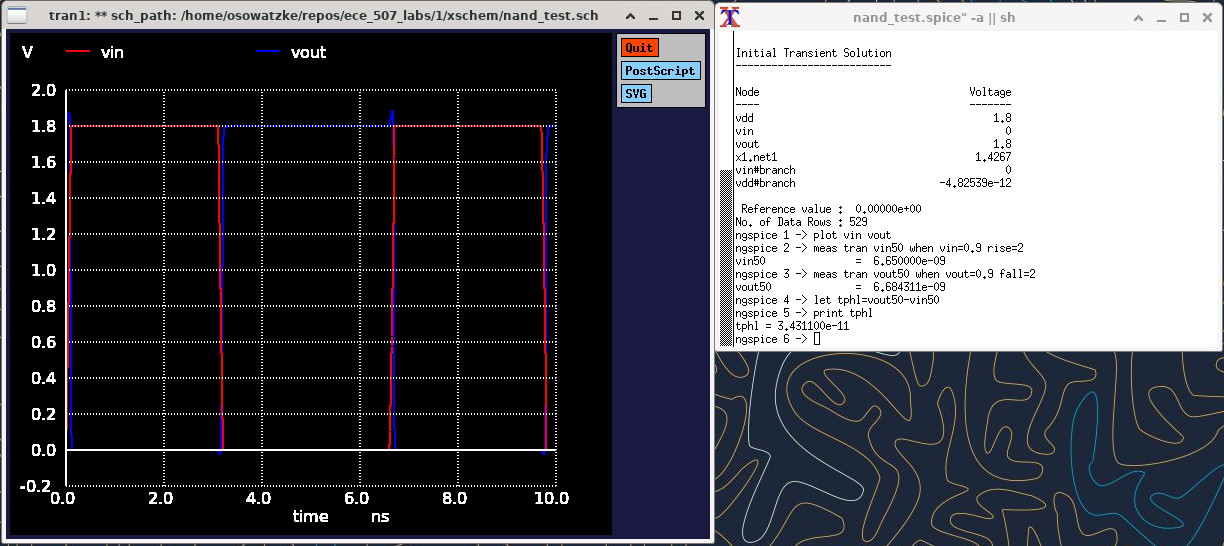
\includegraphics[width=0.8\textwidth]{nand_delay_sweep_vb.png}}
		\caption{\texttt{tphl} Measurement for the NAND Gate when Input Variations are Limited to Input \texttt{b}}
		\label{fig::nand_delay_sweep_vb}
	\end{figure}
	
	Examining the output results, we find that \texttt{tphl = 34.311 ps}. Finally, we can examine the impact of varying both inputs together. The test circuit for this analysis is shown in Figure  \ref{fig::nand_delay_test_sweep_va_vb} and the results are captured in Figure  \ref{fig::nand_delay_sweep_va_vb}.
	
	\begin{figure}[H]
		\centerline{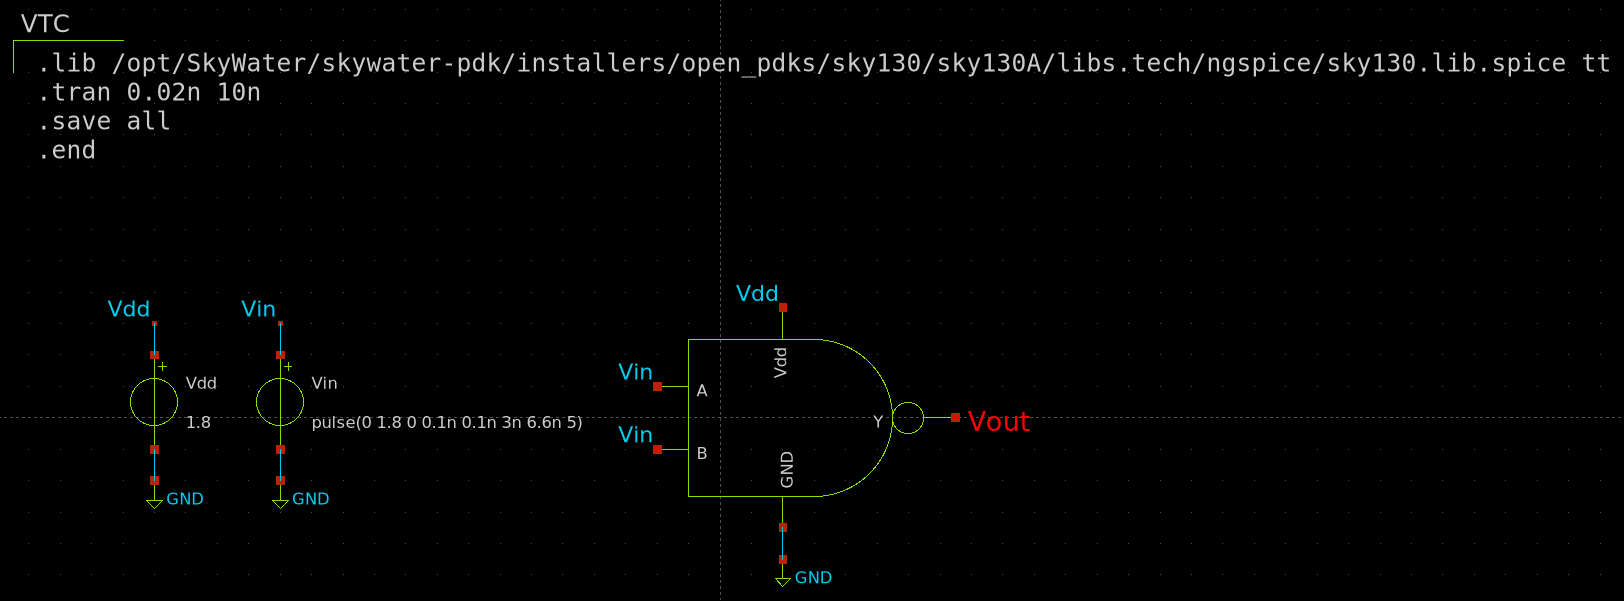
\includegraphics[width=0.8\textwidth]{nand_delay_test_sweep_va_vb.png}}
		\caption{Test Circuit to Measure the Delay of the NAND Gate when Both Inputs are Varied Together}
		\label{fig::nand_delay_test_sweep_va_vb}
	\end{figure}
	
	\begin{figure}[H]
		\centerline{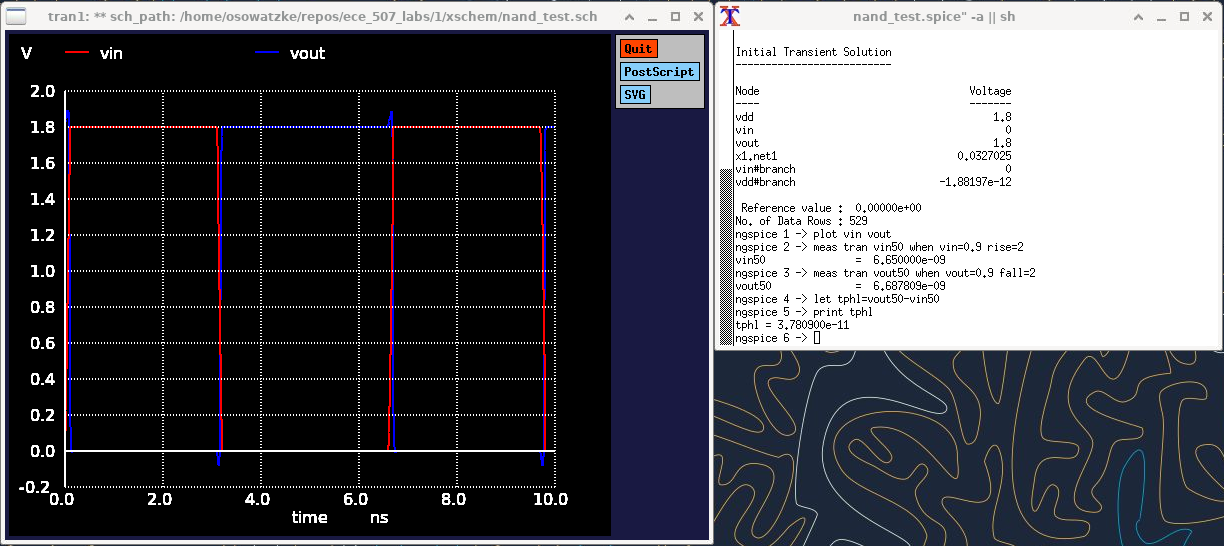
\includegraphics[width=0.8\textwidth]{nand_delay_sweep_va_vb.png}}
		\caption{\texttt{tphl} Measurement for the NAND Gate when Both Inputs are Varied Together}
		\label{fig::nand_delay_sweep_va_vb}
	\end{figure}
	
	Examining the output, we find that \texttt{tphl=37.809 ps}. Note that the delays are data dependent.
	
	\subsection{Power Analysis}
	
	In this section, we analyze the power consumption of our NAND gate. Our test circuit for this analysis is included in Figure \ref{fig::nand_power_test_sweep_va}, and the results of our analysis are shown in Figure \ref{fig::nand_power_sweep_va}.
	
	\begin{figure}[H]
		\centerline{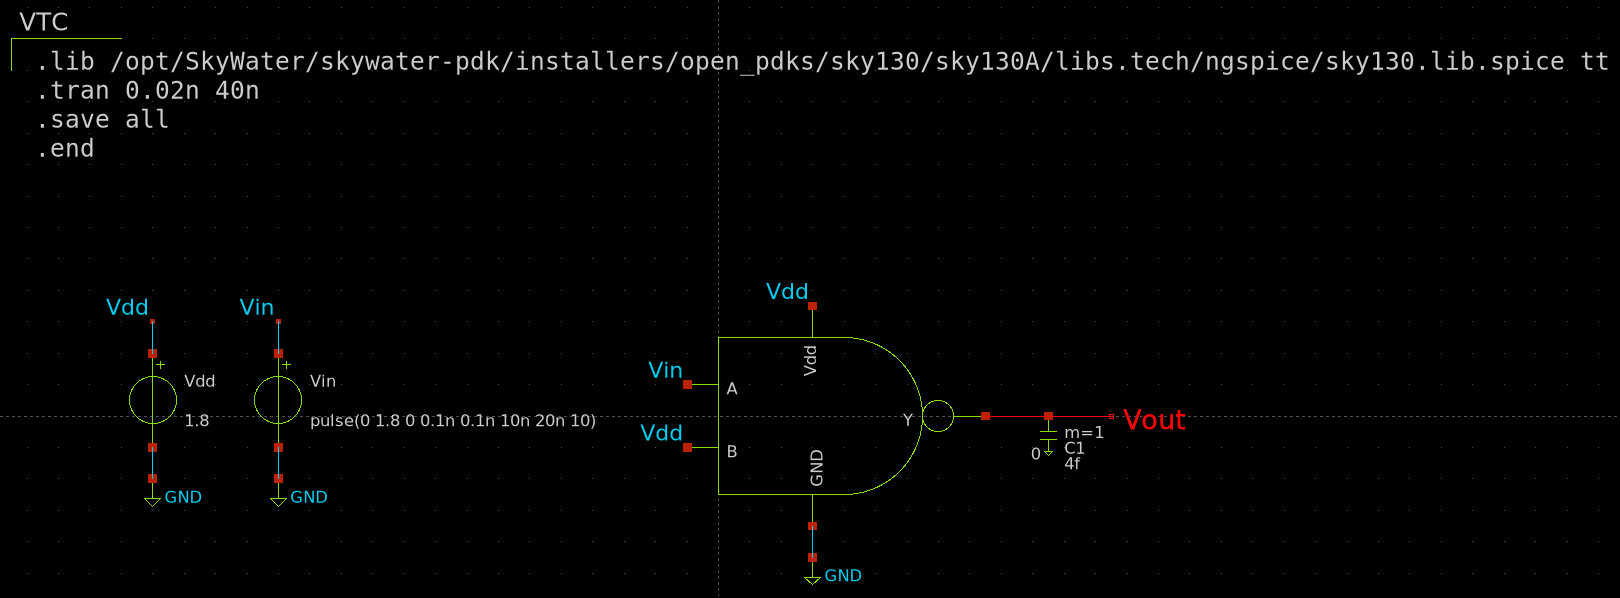
\includegraphics[width=0.8\textwidth]{nand_power_test_sweep_va.png}}
		\caption{Test Circuit to Measure the Power Consumption of the NAND Gate when \texttt{b=1} and Input \texttt{a} is Varied}
		\label{fig::nand_power_test_sweep_va}
	\end{figure}
	
	\begin{figure}[H]
		\centerline{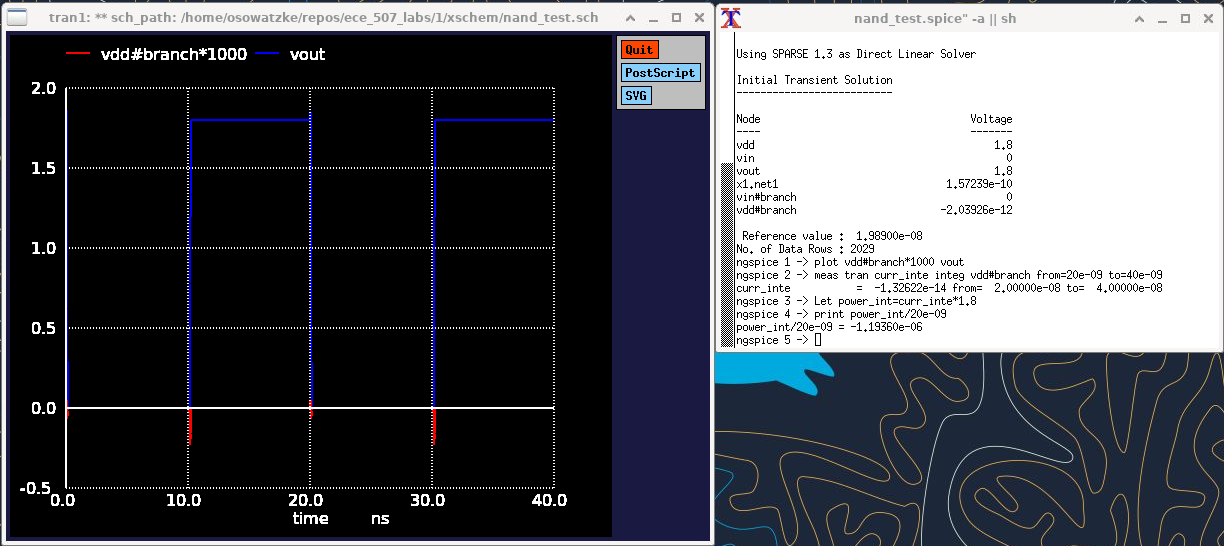
\includegraphics[width=0.8\textwidth]{nand_power_sweep_va.png}}
		\caption{Power Consumption of the NAND Gate wwhen \texttt{b=1} and Input \texttt{a} is Varied}
		\label{fig::nand_power_sweep_va}
	\end{figure}
	
	Examining the results, we find that the power consumption is $1.1936{\mu}W$. We can also measure the power consumption when we fix \texttt{a} at 1 and vary \texttt{b}. The test circuit for this analysis is shown in Figure \ref{fig::nand_power_test_sweep_vb} and the results are shown in Figure \ref{fig::nand_power_sweep_vb}.
	
	\begin{figure}[H]
		\centerline{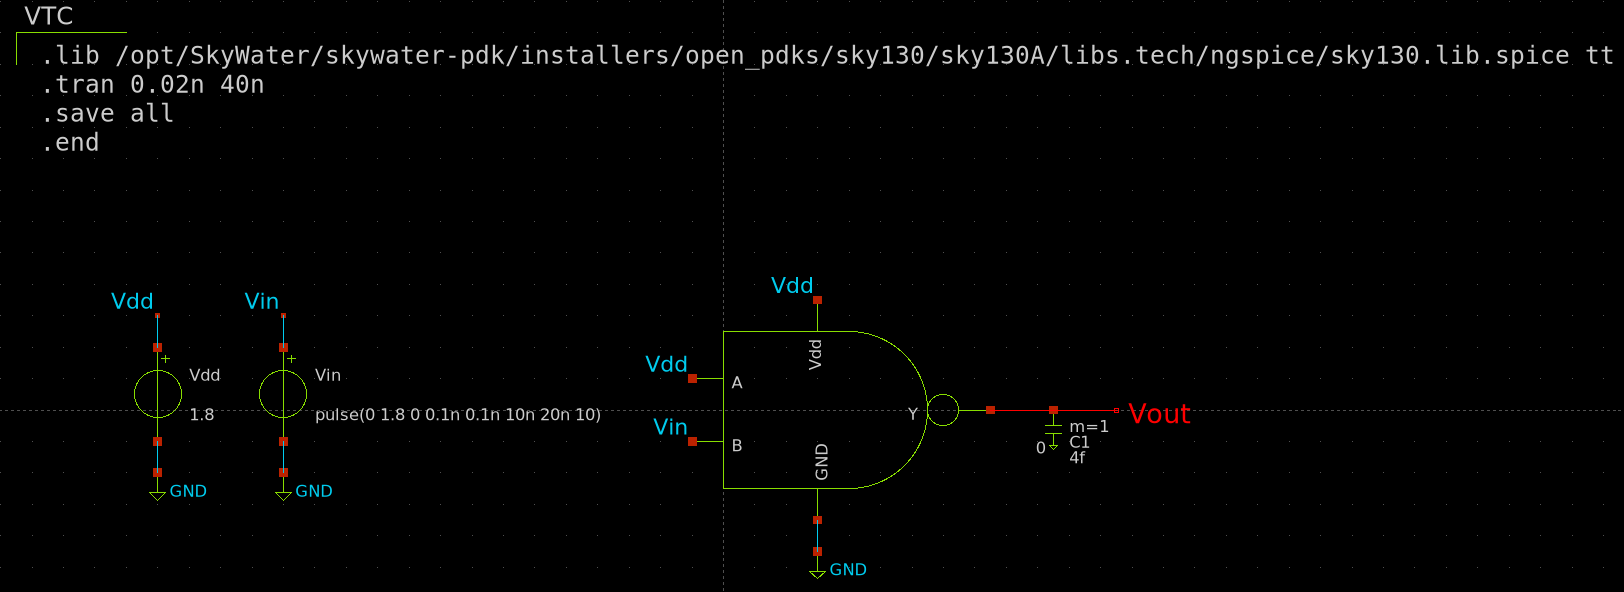
\includegraphics[width=0.8\textwidth]{nand_power_test_sweep_vb.png}}
		\caption{Test Circuit to Measure the Power Consumption of the NAND Gate when \texttt{a=1} and Input \texttt{b} is Varied}
		\label{fig::nand_power_test_sweep_vb}
	\end{figure}
	
	\begin{figure}[H]
		\centerline{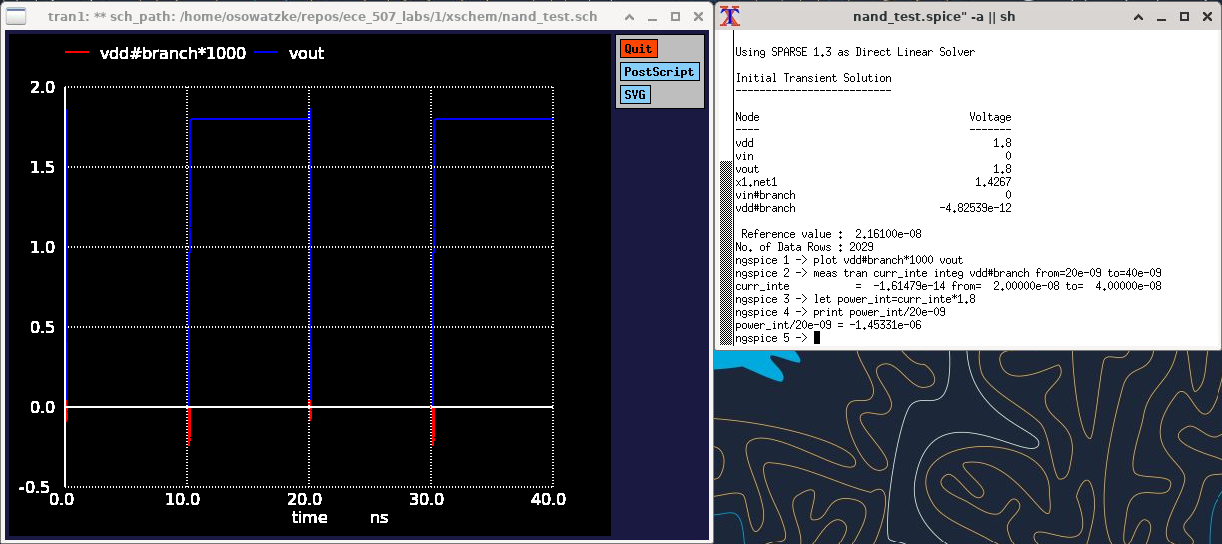
\includegraphics[width=0.8\textwidth]{nand_power_sweep_vb.png}}
		\caption{Power Consumption of the NAND Gate when \texttt{a=1} and Input \texttt{b} is Varied}
		\label{fig::nand_power_sweep_vb}
	\end{figure}
	
	Examining the results, we find that the power consumption is $1.45331{\mu}W$. Next, we measure the power when the inputs are varied together. For this analysis, we use the test circuit shown in Figure \ref{fig::nand_power_test_sweep_va_vb}.
	
	\begin{figure}[H]
		\centerline{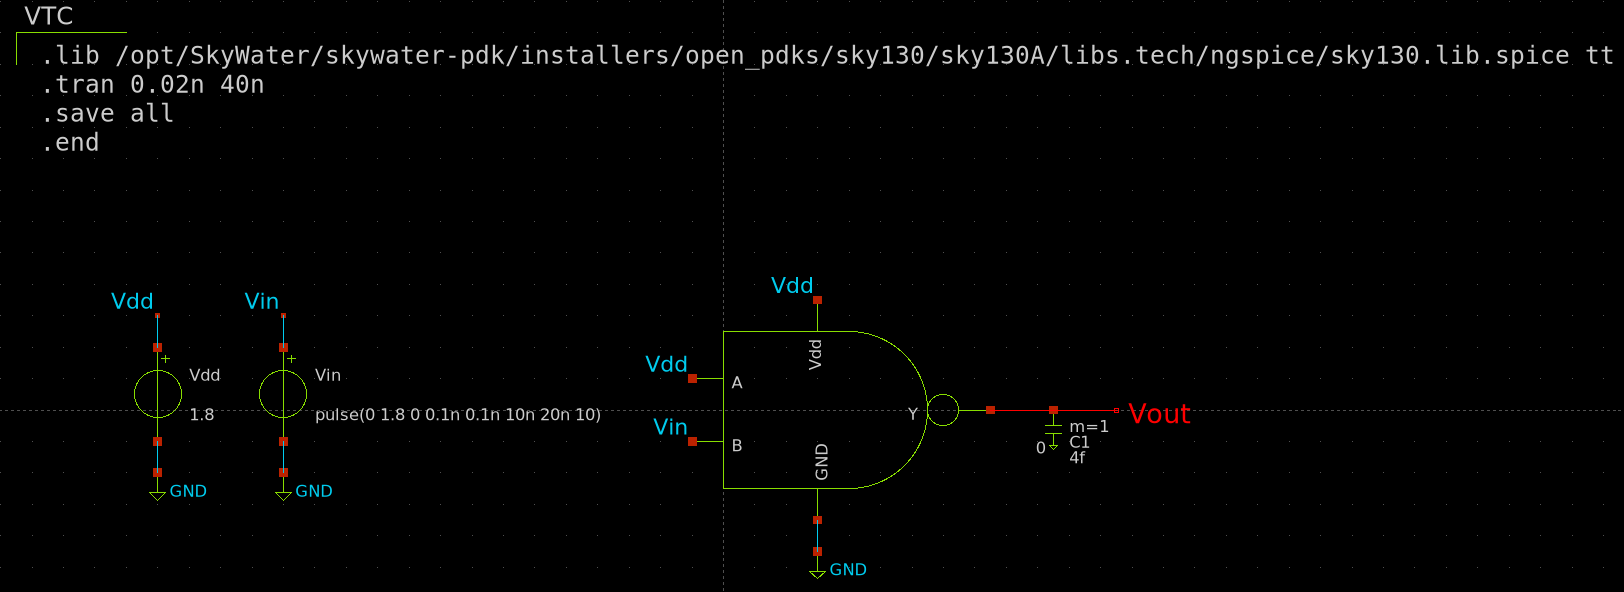
\includegraphics[width=0.8\textwidth]{nand_power_test_sweep_vb.png}}
		\caption{Test Circuit to Measure the Power Consumption of the NAND Gate when Both Inputs are Varied Together}
		\label{fig::nand_power_test_sweep_va_vb}
	\end{figure}
	
	The results of our analysis are included in Figure \ref{fig::nand_power_sweep_vb} and indicate a power consumption of $1.27361{\mu}W$. 
	
	\begin{figure}[H]
		\centerline{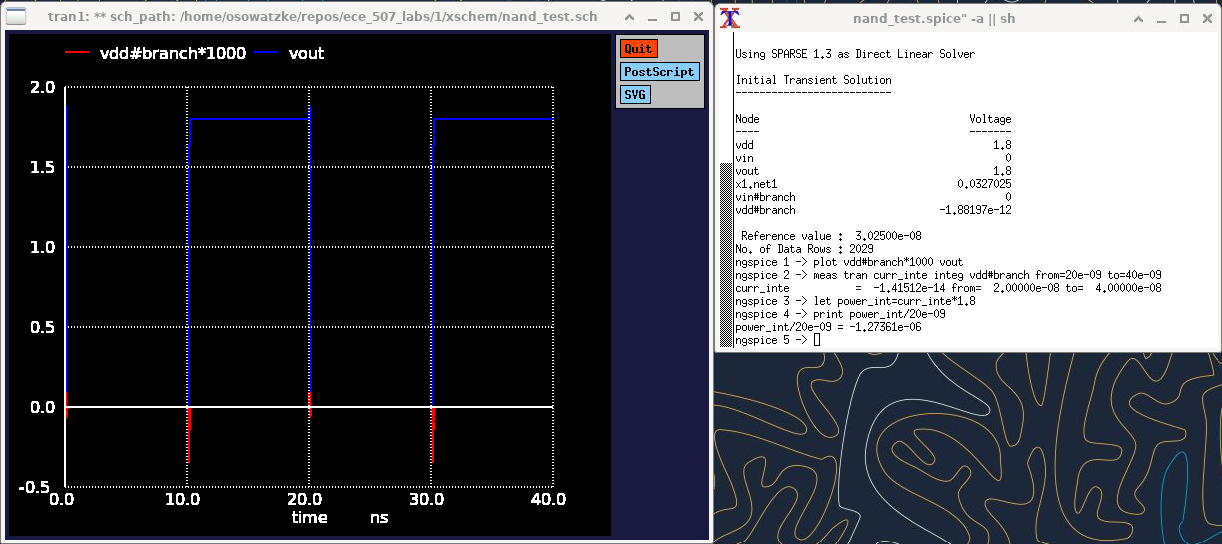
\includegraphics[width=0.8\textwidth]{nand_power_sweep_va_vb.png}}
		\caption{Power Consumption of the NAND Gate when Both Inputs are Varied Together}
		\label{fig::nand_power_sweep_va_vb}
	\end{figure}
	
	\subsection{NOR Gate}
	
	The pull-down circuit of the NAND gate is composed of two parallel NMOS gates. The pull-up circuit is the complement and is composed of two sequential PMOS gates. Note that we also increase the width of the PMOS transistor by a factor of 2 to account for the lower mobility of holes in the p-type material. The schematic for the resulting circuit is shown in Figure \ref{fig::nor_schematic}.
	
	\subsubsection{Design}
	
	\begin{figure}[H]
		\centerline{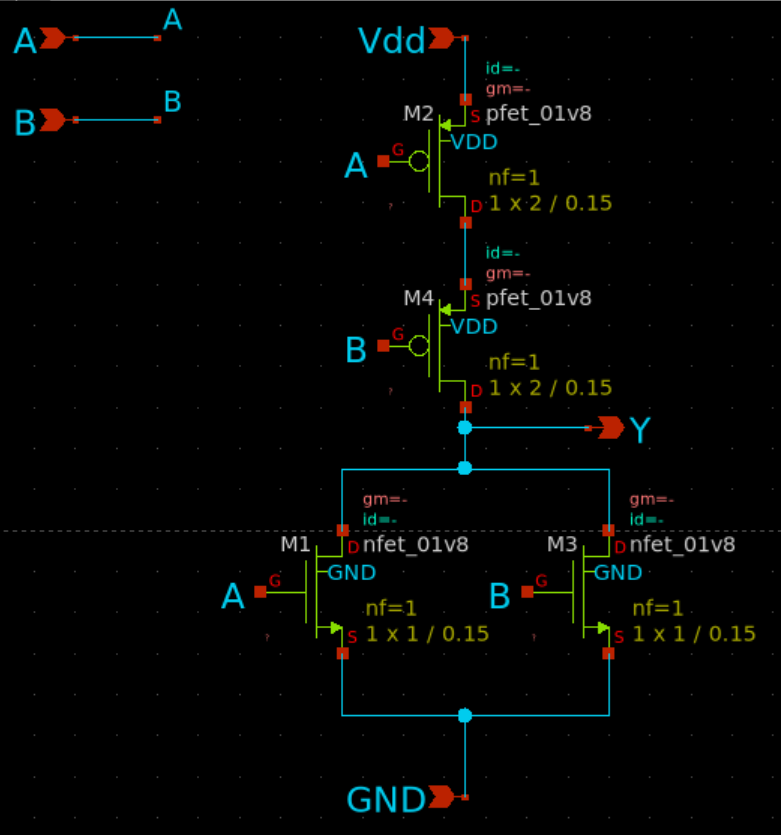
\includegraphics[width=0.4\textwidth]{nor_schematic.png}}
		\caption{NOR Circuit Schematic}
		\label{fig::nor_schematic}
	\end{figure}
	
	We also create a circuit symbol for the NOR gate, which is shown in Figure \ref{fig::nor_symbol}.
	
	\begin{figure}[H]
		\centerline{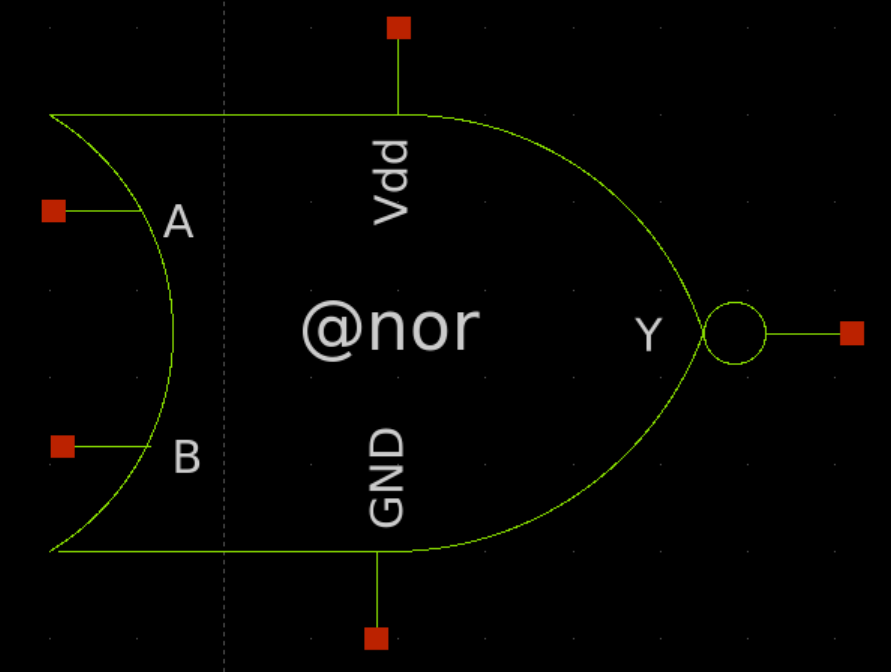
\includegraphics[width=0.4\textwidth]{nor_symbol.png}}
		\caption{NOR Circuit Symbol}
		\label{fig::nor_symbol}
	\end{figure}

	\subsubsection{Voltage Transfer Characteristics}
	
	In this section, we analyze the voltage transfer characteristics (VTC) of our NOR gate. For this analysis, we analyze the VTC when varying \texttt{a} and \texttt{b} independently and when varying \texttt{a} and \texttt{b} together. The test circuit we use when just varying the input \texttt{a} is included in Figure \ref{fig::nor_vtc_test_sweep_va}.
	
	\begin{figure}[H]
		\centerline{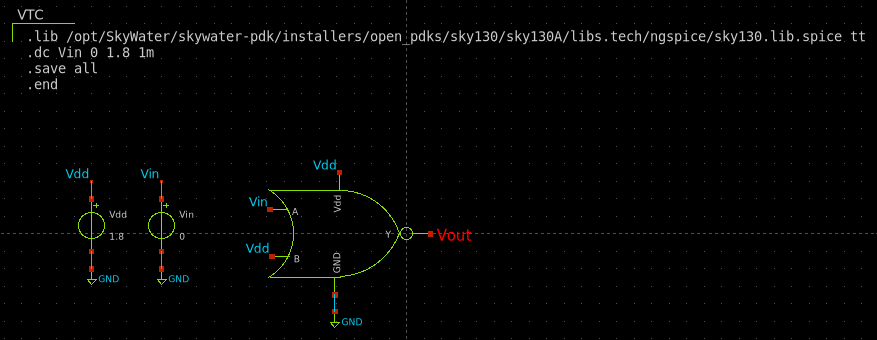
\includegraphics[width=0.8\textwidth]{nor_vtc_test_sweep_va.png}}
		\caption{NOR VTC Test Circuit for Independent Variations of Input \texttt{a}}
		\label{fig::nor_vtc_test_sweep_va}
	\end{figure}
	
	Using this test circuit, we perform DC analysis to determine the VTC and find \texttt{Va}, which is the voltage at which \texttt{Vin = Vout}. The results of this analysis are shown in Figure \ref{fig::nor_vtc_sweep_va}.
	
	\begin{figure}[H]
		\centerline{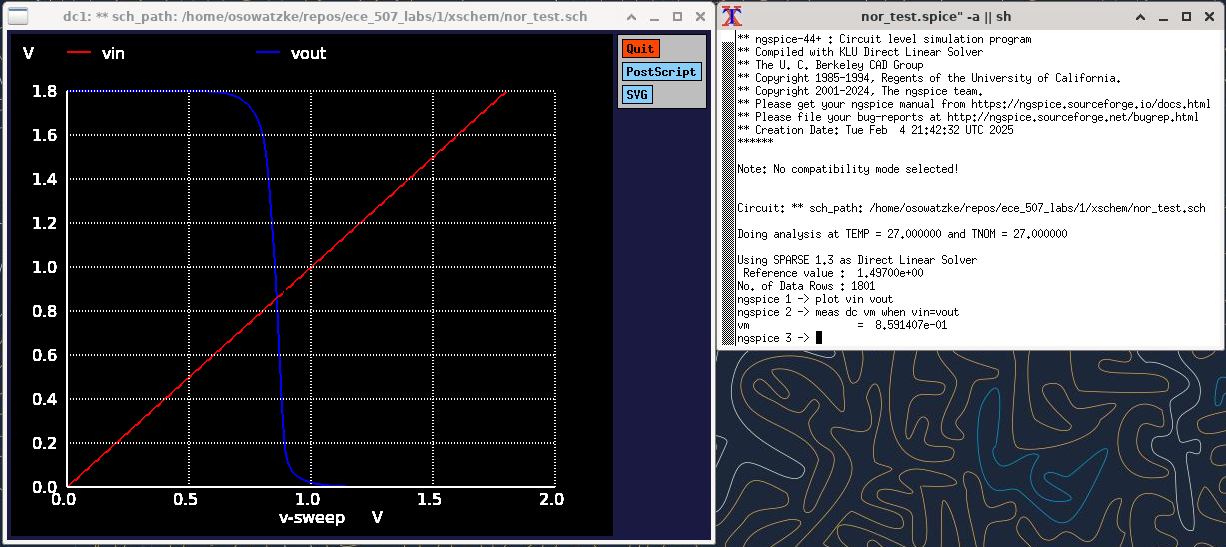
\includegraphics[width=0.8\textwidth]{nor_vtc_sweep_va.png}}
		\caption{NOR VTC Results for Independent Variations of Input \texttt{a}}
		\label{fig::nor_vtc_sweep_va}
	\end{figure}
	
	Examining the results, we find that \texttt{Vm = 0.8591V}. We perform similar analysis for independent variations of the input \texttt{b}. The test circuit and results are attached in figures \ref{fig::nor_vtc_test_sweep_vb} and \ref{fig::nor_vtc_sweep_vb} independently.
	
	\begin{figure}[H]
		\centerline{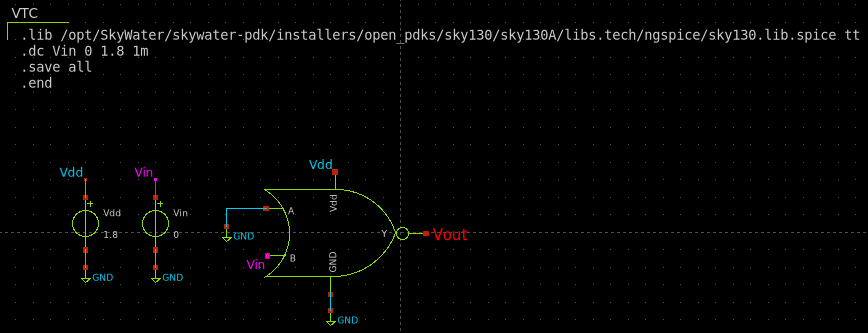
\includegraphics[width=0.8\textwidth]{nor_vtc_test_sweep_vb.png}}
		\caption{NOR VTC Test Circuit for Independent Variations of Input \texttt{b}}
		\label{fig::nor_vtc_test_sweep_vb}
	\end{figure}
	
	\begin{figure}[H]
		\centerline{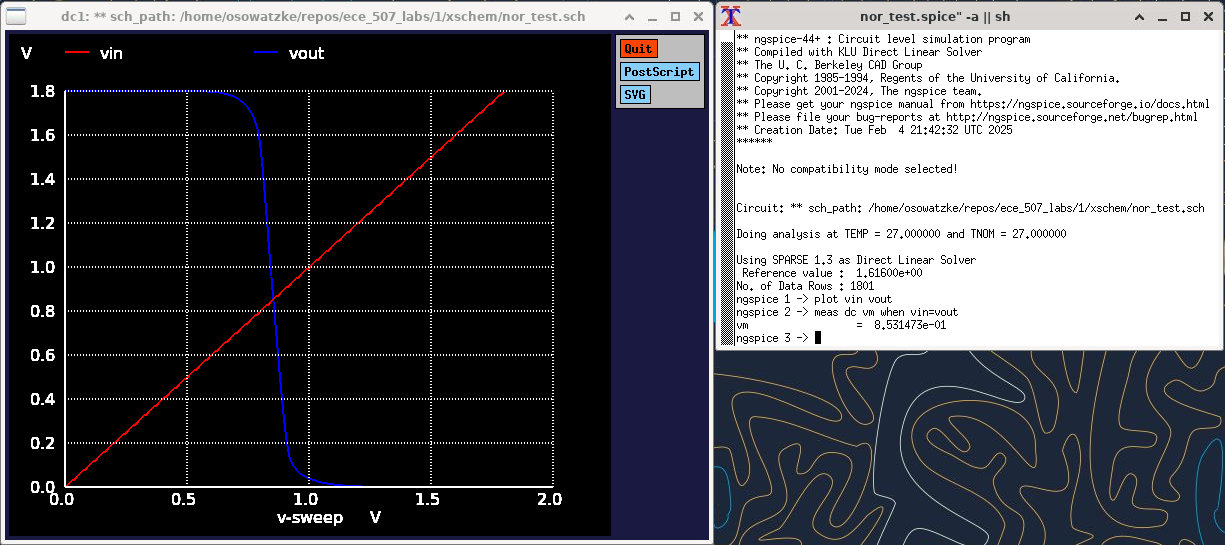
\includegraphics[width=0.8\textwidth]{nor_vtc_sweep_vb.png}}
		\caption{NOR VTC Results for Independent Variations of Input \texttt{b}}
		\label{fig::nor_vtc_sweep_vb}
	\end{figure}
	
	Examining the results, we find that \texttt{Vm = 0.8531V}. Finally, we sweep both inputs \texttt{a} and \texttt{b} together. The test circuit and results for this analysis are included in Figures \ref{fig::nor_vtc_test_sweep_va_vb} and \ref{fig::nor_vtc_sweep_va_vb} respectively.
	
	\begin{figure}[H]
		\centerline{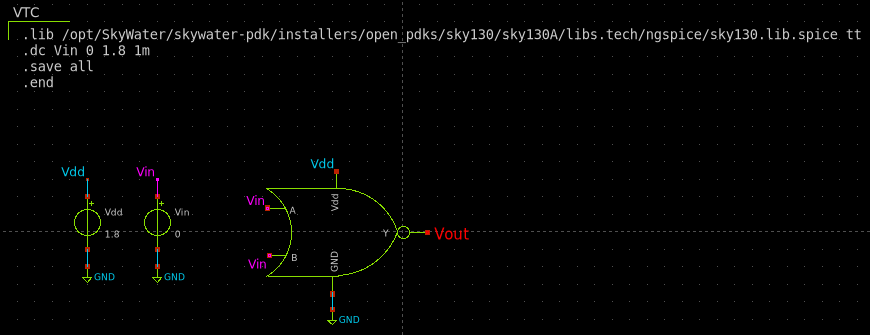
\includegraphics[width=0.8\textwidth]{nor_vtc_test_sweep_va_vb.png}}
		\caption{NOR VTC Test Circuit for Joint Variations of Inputs \texttt{a} and \texttt{b}}
		\label{fig::nor_vtc_test_sweep_va_vb}
	\end{figure}
	
	\begin{figure}[H]
		\centerline{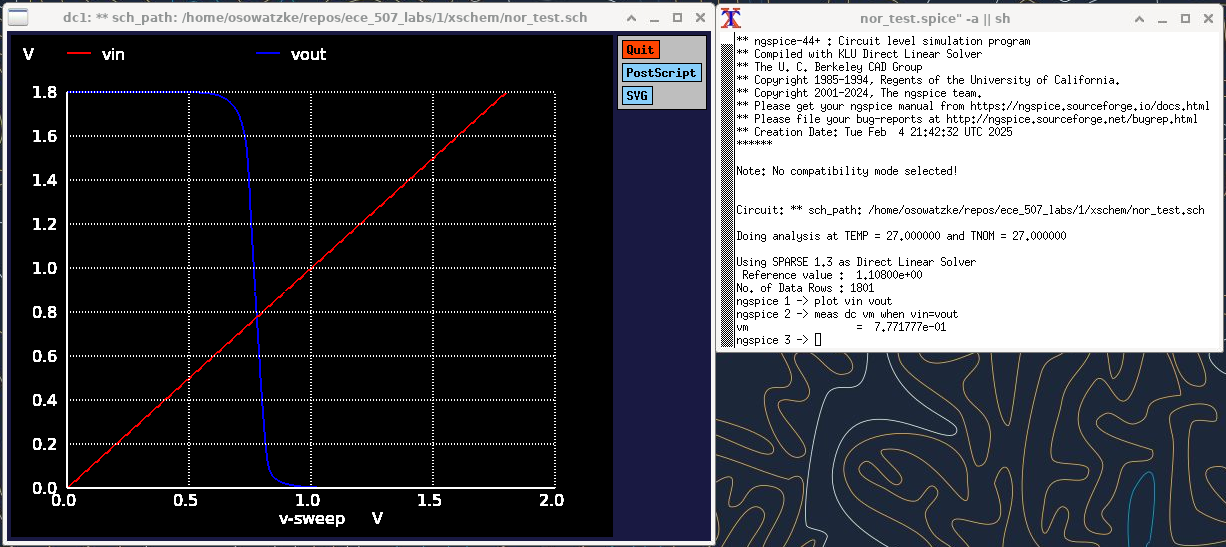
\includegraphics[width=0.8\textwidth]{nor_vtc_sweep_va_vb.png}}
		\caption{NOR VTC Results for Joint Variations of Inputs \texttt{a} and \texttt{b}}
		\label{fig::nor_vtc_sweep_va_vb}
	\end{figure}
	
	Examining the results, we find that \texttt{Vm = 0.7772V}.
	
	\subsection{NAND Gate}

	\begin{align}
		I_{ds_p} &= -k_p\frac{W_p}{L}V_{dsat_p}\left(V_{gs_p} - V_{T0_p} - \frac{V_{dsat_p}}{2}\right)\left(1 + {\lambda_p}V_{ds_p}\right) \\
		&= -k_p\frac{W}{L}V_{dsat_p}\left(V_m - V_{dd} - V_{T0_p} - \frac{V_{dsat_p}}{2}\right)\left(1 + {\lambda_p}(V_m - V_{dd})\right)
	\end{align}
	
	\begin{align}
		I_{ds_n} &= k_n\frac{W_n}{L}V_{dsat_n}\left(V_{gs_n} - V_{T0_n} - \frac{V_{dsat_n}}{2}\right)\left(1 + {\lambda_n}V_{ds_n}\right) \\
		&= k_n\frac{W_n}{L}V_{dsat_n}\left(V_m - V_{T0_n} - \frac{V_{dsat_n}}{2}\right)\left(1 + {\lambda_n}V_m\right)
	\end{align}
	
	Using KCL, we know that:
	
	\begin{equation}
		I_{ds_n} + I_{ds_p} = 0
	\end{equation}
	
	Solving numerically, using the parameters in Table \ref{table::nmos_params} we find that $V_m = 0.8422 V$.
	
	
\end{document}